%%%%%%%%%%%%%%%%%%%%%%%%%%%%%%%%%%%%%%%%%
% Beamer Presentation
% LaTeX Template
% Version 1.0 (10/11/12)
%
% This template has been downloaded from:
% http://www.LaTeXTemplates.com
%
% License:
% CC BY-NC-SA 3.0 (http://creativecommons.org/licenses/by-nc-sa/3.0/)
%
%%%%%%%%%%%%%%%%%%%%%%%%%%%%%%%%%%%%%%%%%

%----------------------------------------------------------------------------------------
%	PACKAGES AND THEMES
%----------------------------------------------------------------------------------------

\documentclass{beamer}

\mode<presentation> {

% The Beamer class comes with a number of default slide themes
% which change the colors and layouts of slides. Below this is a list
% of all the themes, uncomment each in turn to see what they look like.

%\usetheme{default}
%\usetheme{AnnArbor}
%\usetheme{Antibes}
%\usetheme{Bergen}
%\usetheme{Berkeley}
%\usetheme{Berlin}
%\usetheme{Boadilla}
%\usetheme{CambridgeUS}
%\usetheme{Copenhagen}
%\usetheme{Darmstadt}
%\usetheme{Dresden}
\usetheme{Frankfurt}
%\usetheme{Goettingen}
%\usetheme{Hannover}
%\usetheme{Ilmenau}
%\usetheme{JuanLesPins}
%\usetheme{Luebeck}
%\usetheme{Madrid}
%\usetheme{Malmoe}
%\usetheme{Marburg}
%\usetheme{Montpellier}
%\usetheme{PaloAlto}
%\usetheme{Pittsburgh}
%\usetheme{Rochester}
%\usetheme{Singapore}
%\usetheme{Szeged}
%\usetheme{Warsaw}

% As well as themes, the Beamer class has a number of color themes
% for any slide theme. Uncomment each of these in turn to see how it
% changes the colors of your current slide theme.

%\usecolortheme{albatross}
%\usecolortheme{beaver}
%\usecolortheme{beetle}
%\usecolortheme{crane}
%\usecolortheme{dolphin}
%\usecolortheme{dove}
%\usecolortheme{fly}
%\usecolortheme{lily}
%\usecolortheme{orchid}
%\usecolortheme{rose}
%\usecolortheme{seagull}
%\usecolortheme{seahorse}
%\usecolortheme{whale}
%\usecolortheme{wolverine}

%\setbeamertemplate{footline} % To remove the footer line in all slides uncomment this line
%\setbeamertemplate{footline}[page number] % To replace the footer line in all slides with a simple slide count uncomment this line

%\setbeamertemplate{navigation symbols}{} % To remove the navigation symbols from the bottom of all slides uncomment this line
}

\usepackage{graphicx} % Allows including images
\usepackage{booktabs} % Allows the use of \toprule, \midrule and \bottomrule in tables
\usepackage{simplewick}
\usepackage{dsfont}
\usepackage{feynmp-auto}
%       Matthias Paper
        \newcommand{\s}{\small}
        \newcommand{\bu}{{\bar u}}
        \newcommand{\cD}{{\cal D}}
        \newcommand{\cO}{{\cal O}}
        \newcommand{\cP}{{\cal P}}
        \newcommand{\as}{\alpha_s}
        \newcommand{\wh}{\widehat}
        \newcommand{\nn}{\nonumber}
        \newcommand{\ol}{\overline}
        \newcommand{\wt}{\widetilde}
        \newcommand{\ve}{\varepsilon}
        \newcommand{\IM}{\mbox{\rm Im}}
        \newcommand{\RE}{\mbox{\rm Re}}
        \newcommand{\po}{\phantom{00}}
        \newcommand{\eqn}[1]{(\ref{#1})}
        \newcommand{\mev}{\mbox{\rm MeV}}
        \newcommand{\gev}{\mbox{\rm GeV}}
        \newcommand{\tvs}{\vbox{\vskip 6mm}}
        \newcommand{\mvs}{\vbox{\vskip 8mm}}
        \newcommand{\bmvs}{\vbox{\vskip 10mm}}
        \newcommand{\MSb}{{\overline{\rm MS}}}
        \newcommand{\aGG}{\langle\alpha_s GG\rangle}
        \newcommand{\sfrac}[2]{\mbox{$\frac{#1}{#2}$}}
        \newcommand{\gsim}{~{}_{\textstyle\sim}^{\textstyle >}~}
        \newcommand{\lsim}{~{}_{\textstyle\sim}^{\textstyle <}~}

%----------------------------------------------------------------------------------------
%	TITLE PAGE
%----------------------------------------------------------------------------------------

\title[Anomalous Dimension Matrix]{1-Loop Anomalous Dimensions of 4-Quark Operators} % The short title appears at the bottom of every slide, the full title is only on the title page

\author{Dirk Hornung} % Your name
\institute[IFAE] % Your institution as it will appear on the bottom of every slide, may be shorthand to save space
{
Universitat Autonoma de Barcelona \\ % Your institution for the title page
\medskip
\textit{dirkhornung91@gmail.com} % Your email address
}
\date{\today} % Date, can be changed to a custom date

\begin{document}

\begin{frame}
\titlepage % Print the title page as the first slide
\end{frame}

\begin{frame}
\frametitle{Overview} % Table of contents slide, comment this block out to remove it
\tableofcontents % Throughout your presentation, if you choose to use \section{} and \subsection{} commands, these will automatically be printed on this slide as an overview of your presentation
\end{frame}

%----------------------------------------------------------------------------------------
%	PRESENTATION SLIDES
%----------------------------------------------------------------------------------------

%------------------------------------------------
\section{Introduction} % Sections can be created in order to organize your presentation into discrete blocks, all sections and subsections are automatically printed in the table of contents as an overview of the talk
%------------------------------------------------
\subsection{Introduction}
\begin{frame}
\frametitle{Introduction}
\Huge{\centerline{Introduction}} 
\end{frame}

\begin{frame}
\frametitle{Two Point Correlation Function}
Two point correlation function:
\begin{equation*}
\begin{split}
	\Pi_{\mu\nu}^{V/A}(q) \,&\equiv\, i\!\int\! {\rm d}x\, {\rm e}^{iqx}\,
	\langle\Omega|T\{ j_\mu^{V/A}(x) j_\nu^{V/A}(0)^\dagger\}|\Omega\rangle \\
	&=\, \big( q_\mu q_\nu - g_{\mu\nu} q^2 \big  )\, \Pi^{V/A}(q^2) \,,
\end{split}
\end{equation*}
where
\begin{equation*}
 j^V_\mu = \bar u \gamma_\mu d (x) \qquad \text{and} \qquad j^A_\mu = \bar u \gamma_\mu \gamma_5 d (x) 
\end{equation*}
Operator product expansion (OPE) :
\begin{equation*}
	\label{ope}
	\Pi^{V/A}(Q^2) \,=\, C_0(Q^2) + C_4(Q^2)\, \frac{\langle O_4 \rangle}{Q^4} +
	C_6^{V/A}(Q^2)\, \frac{\langle O_6 \rangle}{Q^6} + \ldots \,.
\end{equation*}
\end{frame}

\begin{frame}
\frametitle{Wilson-Coefficients}
\tiny
\begin{equation*}
	\label{C6O6VmA}
	C_6^{V-A}(Q^2)\,\langle O_6 \rangle \,=\,
	4\pi^2 a_s \,\Big\{ \Big[\, 2 + \Big( \sfrac{25}{6} - L \Big  ) a_s \Big]
	\langle Q_-^{\,o} \rangle -
	\Big( \sfrac{11}{18} - \sfrac{2}{3} L \Big  ) a_s \langle Q_-^{\,s} \rangle
	\Big\} \,
\end{equation*}
\begin{eqnarray*}
	C_6^{V+A}(Q^2)\,\langle O_6 \rangle \,&=&\,
	-\,4\pi^2 a_s \,\Big\{ \Big[\, 2 + \Big( \frac{155}{24} - \frac{7}{2} L \Big  )
	a_s \Big] \langle Q_+^{\,o} \rangle +
	\Big( \frac{11}{18} - \frac{2}{3} L \Big  ) a_s \langle Q_+^{\,s} \rangle +
	\nn \\
	\mvs
	&& \hspace{17mm}
	\Big[\, \frac{4}{9} + \Big( \frac{37}{36} - \frac{95}{162} L \Big  ) a_s \Big]
	\langle Q_3 \rangle +
	\Big( \frac{35}{108} - \frac{5}{18} L \Big  ) a_s \langle Q_4 \rangle + \nn \\
	\mvs
	&& \hspace{27mm}
	\label{C6O6VpA}
	\Big( \frac{14}{81} - \frac{4}{27} L \Big  ) a_s \langle Q_6 \rangle -
	\Big( \frac{2}{81} + \frac{4}{27} L \Big  ) a_s \langle Q_7 \rangle \,
\end{eqnarray*}
\cite{p1}
\rule{\textwidth}{0.4pt}
\small
with
\begin{equation*}
	a_s \equiv \frac{\alpha_s}{\pi} \qquad \text{and} \qquad L \equiv \ln \frac{Q^2}{\mu^2}
\end{equation*}
\end{frame}

\begin{frame}
\frametitle{Operator Basis}
\tiny
\begin{eqnarray*}
	Q_V^{O} \,&=&\, (\bar u\gamma_\mu t^a d\bar d\gamma^\mu t^a u) \,, \quad
	Q_A^{O} \,=\, (\bar u\gamma_\mu\gamma_5 t^a d\bar d\gamma^\mu\gamma_5 t^a u)
	\,,\\
	Q_V^{S} \,&=&\, (\bar u\gamma_\mu d\bar d\gamma^\mu u) \,, \quad
	Q_A^{S} \,=\, (\bar u\gamma_\mu\gamma_5 d\bar d\gamma^\mu\gamma_5 u) \,, \\
	Q_3 \,&\equiv&\, (\bar u\gamma_\mu t^a u + \bar d\gamma_\mu t^a d)
	\!\sum\limits_{q=u,d,s} (\bar q\gamma^\mu t^a q) \,, \\
	Q_4 \,&\equiv&\, (\bar u\gamma_\mu\gamma_5 t^a u +
	                  \bar d\gamma_\mu\gamma_5 t^a d)
	\!\sum\limits_{q=u,d,s} (\bar q\gamma^\mu\gamma_5 t^a q) \,, \\
	Q_5 \,&\equiv&\, (\bar u\gamma_\mu u + \bar d\gamma_\mu d)
	\!\sum\limits_{q=u,d,s} (\bar q\gamma^\mu q) \,, \\
	Q_6 \,&\equiv&\, (\bar u\gamma_\mu\gamma_5 u + \bar d\gamma_\mu\gamma_5 d)
	\!\sum\limits_{q=u,d,s} (\bar q\gamma^\mu\gamma_5 q) \,, \\
	Q_7 \,&\equiv&\, \sum\limits_{q=u,d,s} (\bar q\gamma_\mu t^a q)
	\!\sum\limits_{q^\prime=u,d,s} (\bar q^\prime\gamma^\mu t^a q^\prime) \,, \\
	Q_8 \,&\equiv&\, \sum\limits_{q=u,d,s} (\bar q\gamma_\mu\gamma_5 t^a q)
	\!\sum\limits_{q^\prime=u,d,s} (\bar q^\prime\gamma^\mu\gamma_5 t^a q^\prime)
	\,, \\
	Q_9 \,&\equiv&\, \sum\limits_{q=u,d,s} (\bar q\gamma_\mu q)
	\!\sum\limits_{q^\prime=u,d,s} (\bar q^\prime\gamma^\mu q^\prime) \,, \\
	Q_{10} \,&\equiv&\, \sum\limits_{q=u,d,s} (\bar q\gamma_\mu\gamma_5 q)
	\!\sum\limits_{q^\prime=u,d,s} (\bar q^\prime\gamma^\mu\gamma_5 q^\prime) \,.
\end{eqnarray*} 
\end{frame}

\begin{frame}
\frametitle{What To Do}
\begin{itemize}
\item Compute amplitudes from operator insertions
\item Find possible contractions (Feynman diagrams) 
\item Extract renormalization constants ($ \hat Z$)
\item Calculate Anomalous dimension matrix ($\gamma^{(1)}$)
\item Check Renormalization Group Equation (RGE)
\end{itemize}
\end{frame}

\begin{frame}
\frametitle{$0^{th}$ Order Diagram}
\small
4-quark operators:
\begin{equation*}
	Q^S_{V,A} = \left ( \bar{q}^A \Gamma_1 q^B \bar q^B \Gamma_2 q^A \right  )  (z) \qquad \text{and} \qquad  Q^O_{V,A} = \left ( \bar{q}^A t^a \Gamma_1 q^B \bar q^B t^a \Gamma_2 q^A \right  )  (z)
\end{equation*}
\vspace{0.5cm}
Green function with operator insertion:
\begin{fmffile}{samplepics}
\begin{equation*}
\begin{gathered}
\begin{fmfgraph*}(75,60)
	\fmfleftn{i}{2} \fmfrightn{o}{2}
	\fmf{fermion, label=$p_3$}{i1,v1}
	\fmf{fermion, label=$p_4$, label.side=right}{v1,o1}
	\fmf{fermion, label=$p_1$, label.side=left}{i2,v1}
	\fmf{fermion, label=$p_2$}{v1,o2}
	\fmfv{decoration.shape=square, decoration.size=6, label=z}{v1}
	\fmflabel{$x_1$}{i2}
	\fmflabel{$x_3$}{i1}
	\fmflabel{$x_2$}{o2}
	\fmflabel{$x_4$}{o1}
\end{fmfgraph*}
\end{gathered}
=	
\bcontraction[1ex]{}{q}{{}^i_\alpha(x_1) \bar q^j_\beta(x_2) [ \bar}{q} 
\contraction[1ex]{q^i_\alpha(x_1) \bar}{q}{{}^j_\beta(x_2) [ \bar q^A \Gamma_1}{q}
q^i_\alpha(x_1) \bar q^j_\beta(x_2) [ \bar q^A \Gamma_1 q^B 
\bcontraction[1ex]{\bar}{q}{{}^B \Gamma_2 q^A ](z)}{q}
\contraction[1ex]{\bar q^B \Gamma_2}{q}{{}^A ](z) q^k_\delta(x_3) \bar}{q}
\bar q^B \Gamma_2 q^A  ](z) q^k_\delta(x_3) \bar q^l_\gamma(x_4) 
\end{equation*}
\end{fmffile}
\vspace{0.5cm}
\begin{equation*}
= \delta^{ij} \delta^{kl} [ S^a(x_1-z) \Gamma_1 S^B(z-x_2) S^B(z-x_2) ]_{\alpha\beta} [ S^B (x_3 - z) \Gamma_2 S^A(z-x_4) ]_{\delta\gamma}
\end{equation*}
\end{frame}

\begin{frame}
\frametitle{$0^{th}$ Order Diagram}
Fourier transform:
\begin{equation*}
	\delta^{ij}\delta^{kl} [S^A(p_1) \Gamma_1 S^B(-p_2)]_{\alpha\beta} [ S^B(p_3) \Gamma_2 S^A(-p_4)  ]_{\delta\gamma}
\end{equation*}
Amputating external propagators:
\begin{equation*}
\begin{split}
	\Gamma^S_{amp} & : \delta^{ij}\delta^{kl} [\Gamma_1]^{AB}_{\alpha\beta} [\Gamma_2]^{BA}_{\delta\gamma} \\
	\Gamma^O_{amp} & : (t^a)^{ij} (t^a)^{kl} [\Gamma_1]^{AB}_{\alpha\beta} [\Gamma_2]^{BA}_{\delta\gamma}	
\end{split}
\end{equation*}
\end{frame}


% ANOMALOUS DIMENSION MATRICES
% ----------------------------
\section{Anomalous Dimension Matrix}

\begin{frame}
\frametitle{Anomalous Dimension Matrix}
\huge\centering
Anomalous Dimension Matrix
\end{frame}


\begin{frame}
\frametitle{Possible Diagrams}
Current-current diagrams:
\begin{figure}
\centering
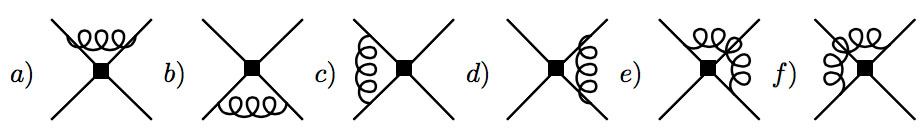
\includegraphics[width=\textwidth]{Figures/currentCurrentDiagrams.jpg}
\end{figure}
Penguin diagrams:
\begin{figure}
\centering
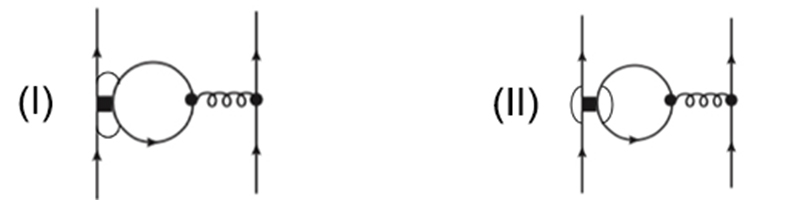
\includegraphics[width=\textwidth]{Figures/penguinDiagrams.jpg}
\end{figure}
\end{frame}

\subsection{V-A Contribution (singlet)}
\begin{frame}
\frametitle{V-A Contribution (singlet)}
\huge\centering
V-A (singlet) 
\end{frame}

\begin{frame}
\frametitle{V-A Contribution (singlet)}	
\small
\begin{align*}
		\Gamma^a &= \frac{\alpha_s}{4\pi} C_F \frac{a}{\epsilon} \delta^{ij} \delta^{kl} [\Gamma_1]^{AB}_{\alpha\beta} [\Gamma_2]^{BA}_{\delta\gamma} \\
		\Gamma^b &= \frac{\alpha_s}{4\pi} C_F \frac{a}{\epsilon} \delta^{ij} \delta^{kl} [\Gamma_1]^{AB}_{\alpha\beta} [\Gamma_2]^{BA}_{\delta\gamma} \\
		\Gamma^c &= \frac{\alpha_s}{4\pi}\frac{1}{\epsilon} (t^b)^{ij}(t^b)^{kl} \left\{ -\frac{1}{4} \left[\gamma_\sigma \gamma_\omega \Gamma_1\right]^{AB}_{\alpha\beta} \left[\gamma^\sigma\gamma^\nu\Gamma_2\right]^{BA}_{\delta\gamma} + (1-a) \left[\Gamma_1\right]^{AB}_{\alpha\beta}\left[\Gamma_2\right]^{BA}_{\delta\gamma}\right\} \\
		\Gamma_d &= \frac{\alpha_s}{4\pi}\frac{1}{\epsilon} (t^b)^{ij} (t^b)^{kl}  \left\{ -\frac{1}{4}\left[\Gamma_1 \gamma_\sigma \gamma_\omega\right]^{AB}_{\alpha\beta} \left[ \Gamma_2 \gamma^\omega \gamma^\sigma \right ]^{BA}_{\delta\gamma} + (1-a) \left[\Gamma_1\right]^{AB}_{\alpha\beta} \left[ \Gamma_2\right ]^{BA}_{\delta\gamma}\right\} \\
		\Gamma^e &= \frac{\alpha_s}{4\pi}\frac{1}{\epsilon}(t^b)^{ij} (t^b)^{kl}  \left\{ \frac{1}{4}\left[ \gamma_\sigma \gamma_\omega \Gamma_1 \right ]^{AB}_{\alpha\beta} \left[\Gamma_2 \gamma^\omega \gamma^\sigma \right]^{BA}_{\delta\gamma}- (1-a) \left[\Gamma_1\right]^{AB}_{\alpha\beta} \left[\Gamma_2\right]^{BA}_{\delta\gamma} \right\}  \\
		\Gamma^f &= \frac{\alpha_s}{4\pi}\frac{1}{\epsilon} (t^b)^{ij}(t^b)^{kl} \left\{\frac{1}{4}\left[\Gamma_1\gamma_\omega \gamma_\sigma\right]^{AB}_{\alpha\beta}\left[\gamma^\sigma\gamma^\omega\Gamma_2\right]^{BA}_{\delta\gamma} -(1-a)\left[\Gamma_1\right]^{AB}_{\alpha\beta} \left[\Gamma_2\right]^{BA}_{\delta\gamma} \right\} 
\end{align*}
\end{frame}

\begin{frame}
\frametitle{V-A Contribution (singlet)}
Vector ($\Gamma_1 = \Gamma_2 = \gamma_\mu$) contribution:
\begin{equation*}
\begin{split}
	\sum_{i=a,\ldots,f}\Gamma^S_{i,V} &= \frac{a_s}{\epsilon} (t^b)^{ij} (t^b)^{kl} \left(-\frac{3}{2}\right) \left[\gamma_5 \gamma_\mu\right]^{AB}_{\alpha\beta} \left[\gamma^\mu \gamma_5 \right]^{BA}_{\delta\gamma} \\
	&= \frac{a_s}{\epsilon}\left(-\frac{3}{2}\right) Q^O_A 
\end{split}
\end{equation*}
Axialvector ($\Gamma_1 = \Gamma_2 = \gamma_\mu\gamma_5$) contribution :
\begin{equation*}
\begin{split}
	 \sum_{i=a,\ldots,f} \Gamma^S_{i,A} &= \frac{a_s}{\epsilon}(t^b)^{ij}(t^b)^{kl}\left(-\frac{3}{2}\right) \left[\gamma_\mu\right]^{AB}_{\alpha\beta} \left[\gamma^\mu\right]^{BA}_{\delta\gamma} \\
&= \frac{a_s}{\epsilon} \left(-\frac{3}{2}\right) Q^O_V
\end{split}
\end{equation*}
\end{frame}

\begin{frame}
\frametitle{V-A Contribution (singlet)}
Noticing:
\begin{equation*}
\begin{split}
	Q^S_V \rightarrow Q^O_A \\
	Q^S_A \rightarrow Q^O_V
\end{split}
\end{equation*}
\begin{equation*}
	Q^S_- \equiv Q^S_V - Q^S_A \rightarrow Q^O_A - Q^O_V = - Q^O_-
\end{equation*}
Total contribution (singlet):
\begin{equation*}
	\sum^S_{i=a,\ldots,f} \Gamma^S_{i,V-A} = \frac{a_s}{\epsilon} \frac{3}{2} Q^O_-.
\end{equation*}
\end{frame}

\begin{frame}
\frametitle{V-A Contribution (singlet)}
Extract renormalization constant:
\begin{equation*}
	\langle q \bar q ( Z^{-1} \vec O^B   ) q \bar q\rangle = \langle q \bar q (\mathds{1} - Z_0^{(1)} \frac{\alpha_s}{\epsilon}) \vec O^R q \bar q \rangle
\end{equation*}
V-A renormalization constants:
\begin{equation*}
	(\hat Z^{(1)}_0)_{21} = \frac{3}{2} \qquad \text{and} \qquad (\hat Z^{(1)}_0)_{22} = 0	
\end{equation*} 
\end{frame}

\subsection{V-A Contribution (octet)}
\begin{frame}
\frametitle{V-A (octet)}
\huge\centering
V-A (octet)
\end{frame}

\begin{frame}
\frametitle{V-A Contribution (octet)}
Colour structures:
\begin{equation*}
t^a t^b \otimes t^a t^b = \frac{C_F}{2N_C}\mathds{1}\otimes\mathds{1} - \frac{1}{N_c}t^a \otimes t^a
\end{equation*}	
\begin{equation*}
t^at^b \otimes t^b t^a = \frac{C_F}{2N_C} \mathds{1} \otimes \mathds{1} + \left( \frac{N_c}{2} - \frac{1}{N_c}\right  ) t^a \otimes t^a
\end{equation*}
\end{frame}

\begin{frame}
\frametitle{V-A Contribution (octet)} 
\begin{equation*}
\begin{split}
	\Gamma^O_a &= \frac{1}{2N_c} \frac{a_s}{4} \frac{a}{\epsilon} Q^O_{V,A}  \\
	\Gamma^O_b &= \frac{1}{2N_c} \frac{a_s}{4} \frac{a}{\epsilon} Q^O_{V,A}  \\
	\Gamma^O_c &= [t^a t^b \otimes t^a t^b ] \left[-\frac{5}{8}Q_{V,A} - \frac{3}{8} Q_{A,V} + (1-a) Q_{V,A}\right]  \\
	\Gamma^O_d &= [t^a t^b \otimes t^a t^b ] \left[-\frac{5}{8}Q_{V,A} - \frac{3}{8} Q_{A,V} + (1-a) Q_{V,A}\right]  \\
	\Gamma^O_e &= \left[ t^a t^b \otimes t^b t^a \right ] \left[\frac{5}{8}Q_{V,A} - \frac{3}{8}Q_{A,V} - (1-a)Q_{V,A}\right]  \\
	\Gamma^O_f &= \left[ t^a t^b \otimes t^b t^a \right ] \left[\frac{5}{8}Q_{V,A} - \frac{3}{8}Q_{A,V} - (1-a)Q_{V,A}\right] 
\end{split}
\end{equation*}
\end{frame}

\begin{frame}
\frametitle{V-A Contribution (octet)}
Total contribution (octet):
\small
\begin{equation*}
\begin{split}
	\sum_{i=a,\ldots,f}\Gamma^O_i = \frac{a_s}{\epsilon} \left[\left(\frac{3}{8} N_c - \frac{a}{4} C_F \right) Q^O_{V,A} - \frac{3}{8}\frac{C_F}{N_c}Q^S_{A,V} + \frac{3}{2} \left( \frac{1}{N_c} - \frac{1}{4} N_c \right ) Q^O_{A,V} \right]
\end{split}
\end{equation*}
\normalsize
Insertion of $Q^O_{V-A}$ in Landau gauge:
\begin{equation*}
	\sum_{i=a,\ldots,f}\Gamma^O_i = \frac{a_s}{\epsilon} \left(\frac{3N_c}{4}-\frac{3}{2N_c}\right) Q^O_{V-A} + \frac{3 C_F}{4 N_C} Q^S_{V-A}
\end{equation*}
Renormalization Constants:
\begin{equation*}
	(\hat Z^{(1)}_0)_{12} = \frac{3N_C}{4} - \frac{3}{2N_C} \qquad \text{and} \qquad  (\hat Z^{(1)}_0)_{12} = \frac{3C_F}{4N_C}
\end{equation*}	
\end{frame}

\begin{frame}
\frametitle{V-A Anomalous Dimension Matrix}
Definition:
\begin{equation*}
	\hat \gamma_O (a_\mu) \equiv Z^{-1}_O(\mu) \mu \frac  {d}{d\mu} \hat Z_O (\mu) 
\end{equation*}
\begin{equation*}
	\hat \gamma^{(1)}_O(a_\mu) = - 2\hat Z^{(1)}_O
\end{equation*}
Anomalous Dimension Matrix (V-A):
\begin{equation*}
	\hat \gamma^{(1)}_{O_{V-A}} = 
	\begin{pmatrix}
		-\frac{3N_C}{2}+\frac{3}{N_C} & -\frac{3C_F}{2N_C} \\
		-3 & 0
	\end{pmatrix}
\end{equation*}
\end{frame}

\subsection{V+A Contribution}
\begin{frame}
\frametitle{V+A Contribution}
\huge\centering
V+A Contribution
\end{frame}

\begin{frame}
\frametitle{V+A Contribution}
Total contribution (singlet):
\begin{equation*}
	\sum_{i=a,\ldots,f} \Gamma^S_{i,(V,A)} = \frac{a_s}{\epsilon} \frac{3}{2} Q^O_{A,V}
\end{equation*}
Total contribution (octet):
\begin{equation*}
	\sum_{a,\ldots,f}\Gamma^{Q^O_+}_{i} = \frac{a_s}{\epsilon} \left[\frac{3 N_c}{8}Q^O_{V,A} - \frac{3 C_F}{4N_c}Q^S_{A,V} - \frac{3}{4}\left(\frac{N_c}{2} - {2}{N_c} \right)Q^O_{A,V}\right]
\end{equation*}
\end{frame}

\begin{frame}
\frametitle{V+A Contribution ($Q^O_+$)}
$Q^O_+$ mixing:
\begin{equation*}
	Q^O_+ = \bar u \gamma_\mu t^a d \bar d \gamma^\mu u + \bar u \gamma_\mu \gamma_5 t^a \bar d \gamma^\mu \gamma_5 t^a u
\end{equation*}
Current-current contribution:
\begin{equation*}
	\sum_{a,\ldots,f}\Gamma^{Q^O_+}_{i} = \frac{a_s}{\epsilon} \left[\frac{3}{2N_c} Q^O_+ - \frac{3 C_F}{4N_c}Q^S_+ \right]
\end{equation*}
\begin{equation*}
	Z_{11} = \frac{3}{2N_c} \qquad \text{and} \qquad Z_{12} = - \frac{3C_F}{4N_c}.
\end{equation*}
\end{frame}

\begin{frame}
\frametitle{V+A Contribution ($Q^O_+$)}
Penguin contribution (singlet case):
\begin{equation*}
\begin{split}
	\Gamma^{Q^S_V}_{amp} &= -\frac{a_s}{6} \left[\frac{1}{\hat \epsilon} - ln \left(\frac{-p^2}{\mu^2}\right) + \frac{2}{3} + \mathcal{O}(\epsilon) \right] \\ 
	&\cdot \left\{ \left[ \gamma^\lambda t^b \right ]^{\bar uu} \sum_q \left[ \gamma_\lambda t^b \right ]^{\bar qq} + \frac{\left[p\!\!\!/ t^b\right]^{\bar uu} \left[p\!\!\!/ t^b\right]^{\bar qq}}{p^2}\right\}
\end{split}
\end{equation*}
Same for vector ($\gamma_\mu$) and axialvector ($\gamma_\mu \gamma_5$):
\begin{equation*}
	\Gamma^{Q^S_{V+A}}_{amp}(local) = - \frac{a_s}{3}\frac{1}{\hat \epsilon} \left[ [\gamma_\lambda t^a]^{\bar uu} [\gamma^\lambda t^a]^{\bar qq}  \right ] + \mathcal{O}(1).
\end{equation*}
Mixing into:
\begin{equation*}
	Q_3 = (\bar u\gamma_\mu t^a u + \bar d \gamma_\mu t^a) \sum_{q=u,d,s} (\bar q \gamma^\mu t^a q).  	
\end{equation*}
\end{frame}

\begin{frame}
\frametitle{V+A Contribution ($Q^O_+$)}
Penguin contribution (octet case):
\begin{equation*}
	t^a \rightarrow t^at^bt^a = -\frac{1}{2N_c},
\end{equation*}
\begin{equation*}
	Z_{13} = \frac{1}{6N_c}. 
\end{equation*}
Anomalous dimension:
\begin{equation*}
	\gamma_{Q^O_+} = 
	\begin{pmatrix}
		-\frac{3}{N_c} & \frac{3C_F}{2N_c} & - \frac{1}{3N_c} & 0 & 0 & 0 & 0 & 0 & 0
	\end{pmatrix}
\end{equation*}
\end{frame}

\begin{frame}
\frametitle{V+A Contribution ($Q^S_+$)}
$Q^S_+$ mixing:
\begin{equation*}
	Q^S_+ = \bar u \gamma_\mu d \bar d \gamma_\mu u + \bar u \gamma_\mu \gamma_5 d \bar d \gamma_\mu \gamma_5 u
\end{equation*}
\begin{equation*}
	 \Gamma^{Q^S_+} = -\frac{a_s}{\epsilon} \frac{3}{2} Q^O_{+} \qquad \text{and} \qquad \Gamma^{Q^S_+}_{pen} = -\frac{1}{3} \frac{a_s}{\epsilon}  
\end{equation*}
Renormalization constants:
\begin{equation*}
	Z_{21} = -\frac{3}{2} \qquad \text{and} \qquad Z_{23} = -\frac{1}{3}
\end{equation*}
Anomalous dimension:
\begin{equation*}
	\gamma_{Q^S_+} = 
	\begin{pmatrix}
		3 & 0 & \frac{2}{3} & 0 & 0 & 0 & 0 & 0 & 0
	\end{pmatrix}
\end{equation*}
\end{frame}

\begin{frame}
\frametitle{V+A Contribution ($Q_3$)}
$Q_3$ mixing:
\begin{equation*}
	Q_3 = (\bar u\gamma_\mu t^a u + \bar d \gamma_\mu t^a) \sum_{q=u,d,s} (\bar q \gamma^\mu t^a q).  	
\end{equation*}
Current-current contribution:
\begin{equation*}
	\sum_{a,\ldots,f} \Gamma_i = \frac{a_s}{\epsilon} \left[\frac{3N_c}{8}Q_3 - \frac{3C_F}{4N_c}Q_6 - \frac{3}{4}\left(\frac{N_c}{2} - \frac{2}{N_c}\right)Q_4 \right]
\end{equation*}
\end{frame}

\begin{frame}
\frametitle{V+A Contribution ($Q_3$)}
\begin{figure}
\centering
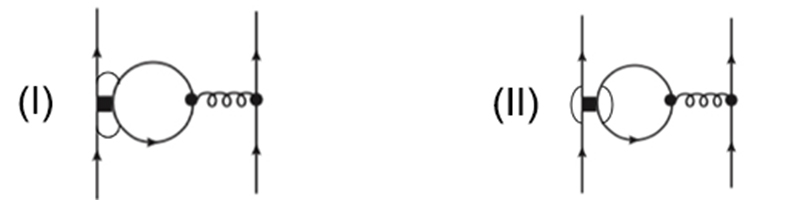
\includegraphics[width=\textwidth]{Figures/penguinDiagrams.jpg}
\end{figure}
\begin{equation*}
	\Gamma^{(1)}_{pen} =
%	-------------------------
	\contraction{}{q}{(x_1) \bar q(x_2) [\bar}{q}
	\bcontraction{q(x_1) \bar}{q}{(x_2) [\bar q q \bar q}{q}
	\contraction{q(x_1) \bar q(x_2) [\bar q}{q}{\bar q q](z) q(x_3) \bar q(x_4) [B \bar}{q}
	\bcontraction[2ex]{q(x_1) \bar q(x_2) [\bar q q \bar}{q}{q](z) q(x_3) \bar q(x_4) [B \bar q}{q}
	\contraction[3ex]{q(x_1) \bar q(x_2) [\bar q q \bar q q](z)}{q}{(x_3) \bar q(x_4) [B \bar q q](y_1) [B \bar}{q}
	\contraction[2ex]{q(x_1) \bar q(x_2) [\bar q q \bar q q](z) q(x_3) \bar}{q}{(x_4) [B \bar q q](y_1) [B \bar q}{q}
	\contraction{q(x_1) \bar q(x_2) [\bar q q \bar q q](z) q(x_3) \bar q(x_4) [}{B}{\bar q q](y_1) [}{B}
% 	---------------------------------
	q(x_1) \bar q(x_2) [\bar q q \bar q q](z) q(x_3) \bar q(x_4) [B \bar q q](y_1) [B \bar q q](y_2),
\end{equation*}
\begin{equation*}	
	\Gamma^{(2)}_{pen} =
%	-------------------------
	\contraction{}{q}{(x_1) \bar q(x_2) [\bar}{q}
	\bcontraction{q(x_1) \bar}{q}{(x_2) [\bar q}{q}
	\bcontraction[2ex]{q(x_1) \bar q(x_2) [\bar q q \bar}{q}{q](z) q(x_3) \bar q(x_4) [B \bar q}{q}
	\bcontraction{q(x_1) \bar q(x_2) [\bar q q \bar q}{q}{](z) q(x_3) \bar q(x_4) [B \bar}{q}
	\contraction[3ex]{q(x_1) \bar q(x_2) [\bar q q \bar q q](z)}{q}{(x_3) \bar q(x_4) [B \bar q q](y_1) [B \bar}{q}
	\contraction[2ex]{q(x_1) \bar q(x_2) [\bar q q \bar q q](z) q(x_3) \bar}{q}{(x_4) [B \bar q q](y_1) [B \bar q}{q}
	\contraction{q(x_1) \bar q(x_2) [\bar q q \bar q q](z) q(x_3) \bar q(x_4) [}{B}{\bar q q](y_1) [}{B}
% 	---------------------------------
	q(x_1) \bar q(x_2) [\bar q q \bar q q](z) q(x_3) \bar q(x_4) [B \bar q q](y_1) [B \bar q q](y_2),
\end{equation*}
\end{frame}

\begin{frame}
\frametitle{V+A Contribution ($Q_3$)}
\tiny
\begin{equation*}
	\Gamma_{\bar qq} =
	\contraction[2ex]{}{q}{(x_1) \bar q(x_2) [( \bar u}{q}{}
	\contraction{q(x_1) \bar}{q}{(x_2) [( \bar }{q}{}
	\bcontraction[2ex]{q(x_1) \bar q(x_2) [( \bar u u + \bar d d  )   \sum \bar }{q}{q](z) q(x_3) \bar q(x_4) [\sum \bar q}{q}
	\bcontraction{q(x_1) \bar q(x_2) [( \bar u u + \bar d d  ) \sum   \bar q }{q}{](z) q(x_3) \bar q(x_4) [\sum \bar }{q}
	\contraction[2ex]{q(x_1) \bar q(x_2) [( \bar u u + \bar d d  )   \sum \bar q q](z) }{q}{(x_3) \bar q(x_4) [\sum \bar q q](y_1) [\sum \bar }{q}
	\contraction{q(x_1) \bar q(x_2) [( \bar u u + \bar d d  ) \sum   \bar q q](z) q(x_3) \bar }{q}{(x_4) [\sum \bar q q](y_1) [\sum \bar q}{q}
	q(x_1) \bar q(x_2) [( \bar u u + \bar d d  ) \sum \bar q q](z)   q(x_3) \bar q(x_4) [\sum \bar q q](y_1) [\sum \bar q q](y_2).
\end{equation*}
\begin{equation*}
	\Gamma_{\bar uu} = 
	\contraction[2ex]{}{q}{(x_1) \bar q(x_2) [( \bar u u + \bar d d  ) \sum \bar }{q}{}
	\contraction{q(x_1) \bar}{q}{(x_2) [( \bar u u + \bar d d  ) \sum \bar q }{q}{}
	\bcontraction[2ex]{q(x_1) \bar q(x_2) [( \bar}{u}{u + \bar d d ) \sum \bar q q](z) q(x_3) \bar q(x_4) [\sum \bar q }{q}
	\bcontraction{q(x_1) \bar q(x_2) [( \bar u}{u}{+ \bar d d ) \sum \bar q q](z) q(x_3) \bar q(x_4) [\sum \bar }{q}
	\contraction[2ex]{q(x_1) \bar q(x_2) [( \bar u u + \bar d d  ) \sum \bar q q](z) }{q}{(x_3) \bar q(x_4) [\sum \bar q q](y_1) [\sum \bar }{q}
	\contraction{q(x_1) \bar q(x_2) [( \bar u u + \bar d d  ) \sum \bar q q](z) q(x_3) \bar }{q}{(x_4) [\sum \bar q q](y_1) [\sum \bar q}{q}
	q(x_1) \bar q(x_2) [( \bar u u + \bar d d  ) \sum \bar q q](z) q(x_3) \bar q(x_4) [\sum \bar q q](y_1) [\sum \bar q q](y_2).
\end{equation*}
\begin{equation*}
	\Gamma_{cross} = 
	\contraction[2ex]{}{q}{(x_1) \bar q(x_2) [( \bar}{u}
	\contraction{q(x_1) \bar}{q}{(x_2) [( \bar u u + \bar d d  ) ( \bar u}{u}{}
	\bcontraction{q(x_1) \bar q(x_2) [( \bar u}{u}{+ \bar d d ) ( \bar u u + \bar d d + \bar s s  )](z) q(x_3) \bar q(x_4) [\sum \bar }{q}
	\bcontraction[2ex]{q(x_1) \bar q(x_2) [( \bar u u + \bar d d  ) ( \bar}{u}{u + \bar d d + \bar s s )](z) q(x_3) \bar q(x_4) [\sum \bar q}{q}
	\contraction[2ex]{q(x_1) \bar q(x_2) [( \bar u u + \bar d d  ) ( \bar u u + \bar d d + \bar s s  )](z) }{q}{(x_3) \bar q(x_4) [\sum \bar q q](y_1) [\sum \bar }{q}
	\contraction{q(x_1) \bar q(x_2) [( \bar u u + \bar d d  ) ( \bar u u + \bar d d + \bar s s  )](z) q(x_3) \bar }{q}{(x_4) [\sum \bar q q](y_1) [\sum \bar q}{q}
	q(x_1) \bar q(x_2) [( \bar u u + \bar d d  ) ( \bar u u + \bar d d + \bar s s  )](z) q(x_3) \bar q(x_4) [\sum \bar q q](y_1) [\sum \bar q q](y_2),
\end{equation*}
\small
\begin{equation*}
	\Gamma_{\bar qq} = - \frac{a_s}{\epsilon} \frac{N_f}{6} Q_3 \qquad \Gamma_{\bar dd} = - \frac{a_s}{\epsilon}\frac{1}{3} Q_7 \qquad \Gamma_{cross} = -\frac{a_s}{\epsilon} \frac{1}{N_c} \frac{1}{6} Q_3
\end{equation*}
\begin{equation*}
	\gamma_{Q3} = 
	(
	\begin{matrix}
		0 & 0 & -\frac{3N_c}{4}+\frac{N_f}{3}-\frac{1}{3N_c} & \frac{3N_c}{4} - \frac{3}{N_c} & \frac{3C_F}{2 N_c} & \frac{2}{3} & 0 & 0 & 0
	\end{matrix}
	)
\end{equation*}
\end{frame}

\begin{frame}
\frametitle{V+A Contribution ($Q_4$)}
$Q_4$ mixing:
\begin{equation*}
	Q_4 = (\bar u \gamma_\mu \gamma_5 t^a u + \bar d \gamma_\mu \gamma_5 d) \sum_{q=u,d,s} (\bar q \gamma^\mu \gamma_5 t^a q)
\end{equation*}
Current-current diagrams:
\begin{equation*}
	\sum_{i=a,\ldots,f}\Gamma_i = \frac{a_s}{\epsilon}\left[\frac{3N_c}{8}Q_4 -\frac{3C_F}{4N_c}Q_5 -\frac{3}{4}\left(\frac{N_c}{2}-\frac{2}{N_c}\right)Q_3\right]
\end{equation*}
\tiny
\begin{equation*}
	(1-\frac{1}{N_c}) Q_2 = 2Q_1 + 2Q_3 + 2Q_4 -\left(1-\frac{1}{N_c}\right)(Q_5 + Q_6)- Q_7 -Q_8 -\left(1-\frac{1}{N_c}\right)\left(\frac{Q_9 + Q_{10}}{2}\right)
\end{equation*}
\begin{equation*}
	\gamma_{Q4} = 
	\left(
	\begin{matrix}
		0 & 0 & \frac{N_f}{3}-\frac{3N_c}{4}-\frac{1}{3N_c} & \frac{3N_c}{4}-\frac{3}{N_c} & -\frac{3C_F}{2N_c} & -\frac{3}{4}-\frac{3}{4N_c} & -\frac{3}{4}-\frac{3}{4N_c} & \frac{3C_F}{4N_c} & \frac{3C_F}{4N_c} \\
	\end{matrix}
	\right
	     )
\end{equation*}
\end{frame}

\begin{frame}
\frametitle{V+A Contribution ($Q_5, \ldots, Q_{10}$)}
\begin{itemize}
\item $Q_5$ linear dependent 
\item $Q_6, \ldots, Q_{10}$ same calculation method
\end{itemize}
\end{frame}

\begin{frame}
\frametitle{Anomalous Dimension Matrix (V+A)}
\tiny
\begin{equation*}
\begin{split}
       \label{eq:anomalousDimensionMatrixVpA}
       \gamma^{(1)}_{Q_+} &= 
       \left(\begin{matrix}
       	-\frac{3}{N_C} & \frac{3C_F}{2N_C} &-\frac{1}{3N_C} & 0   
       	\\
       	3 & 0 & \frac{2}{3} & 0    \\
       	0 & 0 & \frac{N_f}{3}-\frac{3N_c}{4}-\frac{1}{3N_c} & \frac{3N_c}{4}-\frac{3}{N_c}   \\
       	\frac{3}{2}+\frac{3}{2N_c} & -\frac{3C_F}{2N_c} & \frac{3N_c}{4}+\frac{3}{2}-\frac{11}{6N_c} & -\frac{3N_c}{4}+\frac{3}{2}+\frac{3}{2N_c} \\
       	0 & 0 & \frac{11}{3} & 0 \\
       	0 & 0 & 0 & 0 \\
       	0 & 0 & 0 & 0 \\
       	0 & 0 & 0 & 0 \\
       	0 & 0 & 0 & 0 
       \end{matrix} \right. \\
       &\qquad\qquad\qquad\qquad\qquad\qquad \left.\begin{matrix}
       	0 & 0 & 0 & 0 & 0 \\
       	0 & 0 & 0 & 0 & 0 \\
       	\frac{3C_F}{2N_C} & \frac{2}{3} & 0 & 0 & 0 \\
       	-\frac{3C_F}{2N_c} & -\frac{3}{4}-\frac{3}{4N_c} & -\frac{3}{4}-\frac{3}{4N_c} & \frac{3C_F}{4N_c} & \frac{3C_F}{4N_c} \\
       	0 & 0 & 0 & 0 & 0 \\
       	0 & \frac{N_f}{3}+1-\frac{3N_c}{4}-\frac{1}{3N_c} & \frac{3N_c}{4}-\frac{3}{N_c} & 0  & \frac{3C_F}{2N_c} \\
       	0 & \frac{3N_c}{4}-\frac{10}{3N_c} & -\frac{3N_c}{4} & \frac{3C_F}{2N_c} & 0 \\
       	0 & \frac{2}{3} & 3 & 0 & 0 \\
       	0 & \frac{11}{3} & 0 & 0 & 0 
       \end{matrix}\right)
\end{split}
\end{equation*}
\end{frame}

\section{Renormalization Group Equation}
\subsection{Renormalization Group Equation}
\begin{frame}
\frametitle{Renormalization Group Equation}
\huge\centering
Renormalization Group Equation (RGE)
\end{frame}

\begin{frame}
\frametitle{Wilson coefficients}
\tiny
\begin{equation*}
	C_6^{V-A}(Q^2)\,\langle O_6 \rangle \,=\,
	4\pi^2 a_s \,\Big\{ \Big[\, 2 + \Big( \sfrac{25}{6} - L \Big  ) a_s \Big]
	\langle Q_-^{\,o} \rangle -
	\Big( \sfrac{11}{18} - \sfrac{2}{3} L \Big  ) a_s \langle Q_-^{\,s} \rangle
	\Big\} \,,
\end{equation*}
\begin{eqnarray*}
	C_6^{V+A}(Q^2)\,\langle O_6 \rangle \,&=&\,
	-\,4\pi^2 a_s \,\Big\{ \Big[\, 2 + \Big( \sfrac{155}{24} - \sfrac{7}{2} L \Big  )
	a_s \Big] \langle Q_+^{\,o} \rangle +
	\Big( \sfrac{11}{18} - \sfrac{2}{3} L \Big  ) a_s \langle Q_+^{\,s} \rangle +
	\nn \\
	\mvs
	&& \hspace{17mm}
	\Big[\, \sfrac{4}{9} + \Big( \sfrac{37}{36} - \sfrac{95}{162} L \Big  ) a_s \Big]
	\langle Q_3 \rangle +
	\Big( \sfrac{35}{108} - \sfrac{5}{18} L \Big  ) a_s \langle Q_4 \rangle + \nn \\
	\mvs
	&& \hspace{27mm}
	\Big( \sfrac{14}{81} - \sfrac{4}{27} L \Big  ) a_s \langle Q_6 \rangle -
	\Big( \sfrac{2}{81} + \sfrac{4}{27} L \Big  ) a_s \langle Q_7 \rangle \,,
\end{eqnarray*}
\cite{p1}
\rule{\textwidth}{0.4pt}
\small
with
\begin{equation*}
	a_s \equiv \frac{\alpha_s}{\pi} \qquad \text{and} \qquad L \equiv \ln \frac{Q^2}{\mu^2}
\end{equation*}
\end{frame}

\begin{frame}
\frametitle{Renormalization Group Equation}
General term:
\begin{equation*}
	R_O = \vec C^T (\mu) \langle \vec O(\mu) \rangle,
\end{equation*}
Scale independent ($\mu$):
\begin{equation*}
	\left[\mu \frac{d}{d\mu} \vec C^T(\mu) \right] \langle \vec O (\mu) \rangle = -C^T (\mu) \left[\mu \frac{d}{d\mu} \langle \vec O (\mu) \rangle \right]
\end{equation*}
Anomalous dimension definition:
\begin{equation*}
	-\mu\frac{d}{d\mu} \langle \vec O(\mu) \rangle \equiv \hat \gamma_O(a_\mu) \langle \vec O(\mu) \rangle 
\end{equation*}
$\Rightarrow$
\begin{equation*}
	\mu\frac{d}{d\mu} \vec C(\mu) = \hat \gamma^T_O(a_\mu) \vec C(\mu)
\end{equation*}
with
\begin{equation*}
	\mu \frac{d}{d \mu} = \mu \frac{\partial}{\partial \mu} - \beta_1 a_s^2 \frac{\partial}{\partial a_s}
\end{equation*}
\end{frame}

\begin{frame}
\frametitle{Renormalization Group Equation}
RGE equation:
\begin{equation*}
	\mu\frac{d}{d\mu} \vec C(\mu) = \hat \gamma^T_O(a_\mu) \vec C(\mu).
\end{equation*}
V-A case:
\begin{equation*}
	6 a^2_s \pi^2 
\begin{pmatrix}
	\frac{4}{N_c} - 2 N_c \\
	-1 + N_c^{-2}
\end{pmatrix}
\end{equation*}
V+A case:
\tiny
\begin{equation*}
	a^2_s \pi^2
\begin{pmatrix}
	\frac{24}{N_c} & -6 & \frac{6}{N_c^2} & \frac{88}{27 N_c} + \frac{4 N_c}{3} - \frac{16 N_f}{27} & \frac{16}{3N_c} - \frac{4 N_c}{3} & - \frac{4}{3} + \frac{4}{3N_c^2} & - \frac{32}{27} & 0 & 0 & 0
\end{pmatrix}
\end{equation*} 
\end{frame}

\section{Outlook}
\subsection{Outlook}
\begin{frame}
\frametitle{Outlook}
\huge\centering
Outlook
\end{frame}

\begin{frame}
\frametitle{Outlook}
\begin{itemize}
\item Ambiguities in the definition of OPE terms correspond to exponentially suppressed pertubative higher orders.
\item Those ambiguities are reflected in singularities of the Borel transform of the correlator on the real axis (Renormalons).
\item Renormalon structure can be inferred from OPE structure, which includes the anomalous dimensions.
\item Leading order anomalous dimension influence strength of renormalon pole.
\end{itemize}
\end{frame}

\section{References}

\begin{frame}
\footnotesize{
\begin{thebibliography}{99} % beamer does not support bibtex so references must be inserted manually as below
\bibitem[Dirk Hornung, 2015]{p3} Dirk Hornung (2015)
\newblock 1-Loop Anomalous Dimensions of 4-Quark Operators
\newblock \emph{Master Thesis} 
\end{thebibliography}
}
\footnotesize{
\begin{thebibliography}{99} % beamer does not support bibtex so references must be inserted manually as below
\bibitem[L.E. Adam and K.G. Chetyrkin, 1994]{p1} L.E. Adam and K.G. Chetyrkin, (1994)
\newblock Renormalization of four-quark operators and QCD sum rules.
\newblock \emph{Phys. Lett. B329, 129} 
\end{thebibliography}
}
\footnotesize{
\begin{thebibliography}{99} % beamer does not support bibtex so references must be inserted manually as below
\bibitem[M. Benke and M. Jamin, 2012]{p2} M. Beneke and M. Jamin (2008)
\newblock $\alpha_s$ and the $\tau$ hadronic width: fixed-order, contour- improved and higher-order pertubation theory. 
\newblock \emph{Journal of High Energy Physics} 44
\end{thebibliography}
}
\footnotesize{
\begin{thebibliography}{99} % beamer does not support bibtex so references must be inserted manually as below
\bibitem[R.D.C. Miller and B.H.J. McKellar, 1983]{p1} R.D.C. Miller and B.H.J. McKellar, (1983)
\newblock Anomalous Dimension Matrices Of Four Quark Operators.
\newblock \emph{Phys. Rev. D 28 844} 
\end{thebibliography}
}
\end{frame}

\end{document} 
